\documentclass{article}
\usepackage{fancyhdr}
\usepackage{lipsum}  
\usepackage{listings} 
\usepackage{xcolor}   
\usepackage{amsmath}
\usepackage{enumitem}
\usepackage{graphicx}
\usepackage{caption}
\usepackage{verbatim}

% Define macros for title and author
\newcommand{\thetitle}{STAT 641 \\ Homework 6}
\newcommand{\theauthor}{Keegan Smith}

\title{\thetitle}
\author{\theauthor}

\pagestyle{fancy}
\fancyhf{}  % Clear all header and footer fields
\fancyhead[L]{\nouppercase{\rightmark}}
\fancyhead[C]{\thetitle}  % Title in the center
\fancyhead[R]{\theauthor}  % Your name on the right

\lstset{ %
  backgroundcolor=\color{lightgray},   % choose the background color
  basicstyle=\ttfamily\small,          % size of fonts used for the code
  keywordstyle=\color{blue},           % color for keywords
  commentstyle=\color{green},          % color for comments
  stringstyle=\color{red},             % color for strings
  numbers=left,                        % where to put the line-numbers
  numberstyle=\tiny\color{gray},       % style for line-numbers
  stepnumber=1,                        % the step between two line-numbers
  numbersep=5pt,                       % how far the line-numbers are from the code
  frame=single,                        % adds a frame around the code
  rulecolor=\color{black},             % frame color
  breaklines=true,                     % automatic line breaking
  breakatwhitespace=false,             % automatic breaks should only happen at whitespace
  showspaces=false,                    % don't show spaces in the code
  showstringspaces=false,              % don't show spaces in strings
  showtabs=false,                      % don't show tabs in the code
}

\begin{document}

\maketitle
\section*{Problem 1}
\begin{enumerate}
\item To create a reference plot, we must first make it such that the Weibull is a location-scale distribution. We can accomplish this (as outlined in Handout 8) by applying the transformation: \\
\[
X = \log(Y)
\]
so if $X$ follows a log-Weibull distribution, then $Y$ follows a Weibull distribution. \\
The cdf of the log weibull is: \\
\begin{align*}
P(\ln(Y) \leq x) &= P(Y \leq e^x) \\
&= 1 - e^{-(\frac{e^x}{\alpha})^\gamma} \\
&= 1 - e^{-e^{\frac{x - \theta_1}{\theta_2}}}
\end{align*}
We can then solve for the quantile function: \\
\begin{align*}
s &= 1 - e^{-e^{\frac{x - \theta_1}{\theta_2}}} \\
\ln(-s + 1) &= -e^{\frac{x - \theta_1}{\theta_2}} \\
\ln(-\ln(-s + 1)) &= \frac{x - \theta_1}{\theta_2} \\
\theta_2 \cdot \ln(-\ln(-s + 1)) + \theta_1 &= x \\
\end{align*}
Thus we have: \\
\[
Q_z(u) = \ln(-\ln(-u + 1))
\]
We can then make the reference plot with the following R code (continued from the previous R code):
\begin{verbatim}\
x <- c(0.8402, 1.0644, 1.1298, 1.4314, 1.7795, 1.9121, 2.2343, 2.3424, 2.3559, 2.3855,
2.5734, 2.5815, 2.5893, 2.7562, 2.9040, 2.9295, 3.1124, 3.5490, 3.7684, 3.7953,
3.8846, 3.9766, 4.1918, 4.3887, 4.7106, 4.8918, 4.9716, 6.5018, 7.0740, 7.2158)
y = -log(x)
y = sort(y)
n = length(y)
weib= -y
weib= sort(weib)
i= 1:n
ui= (i-.5)/n
QW= log(-log(1-ui))
plot(QW,weib,abline(lm(weib~QW)),
main="Weibull Reference Plot",cex=.75,lab=c(7,11,7),
xlab="Q=ln(-ln(1-ui))",
ylab="y=ln(W(i))")
\end{verbatim}
\begin{figure}[htbp]
    \centering
    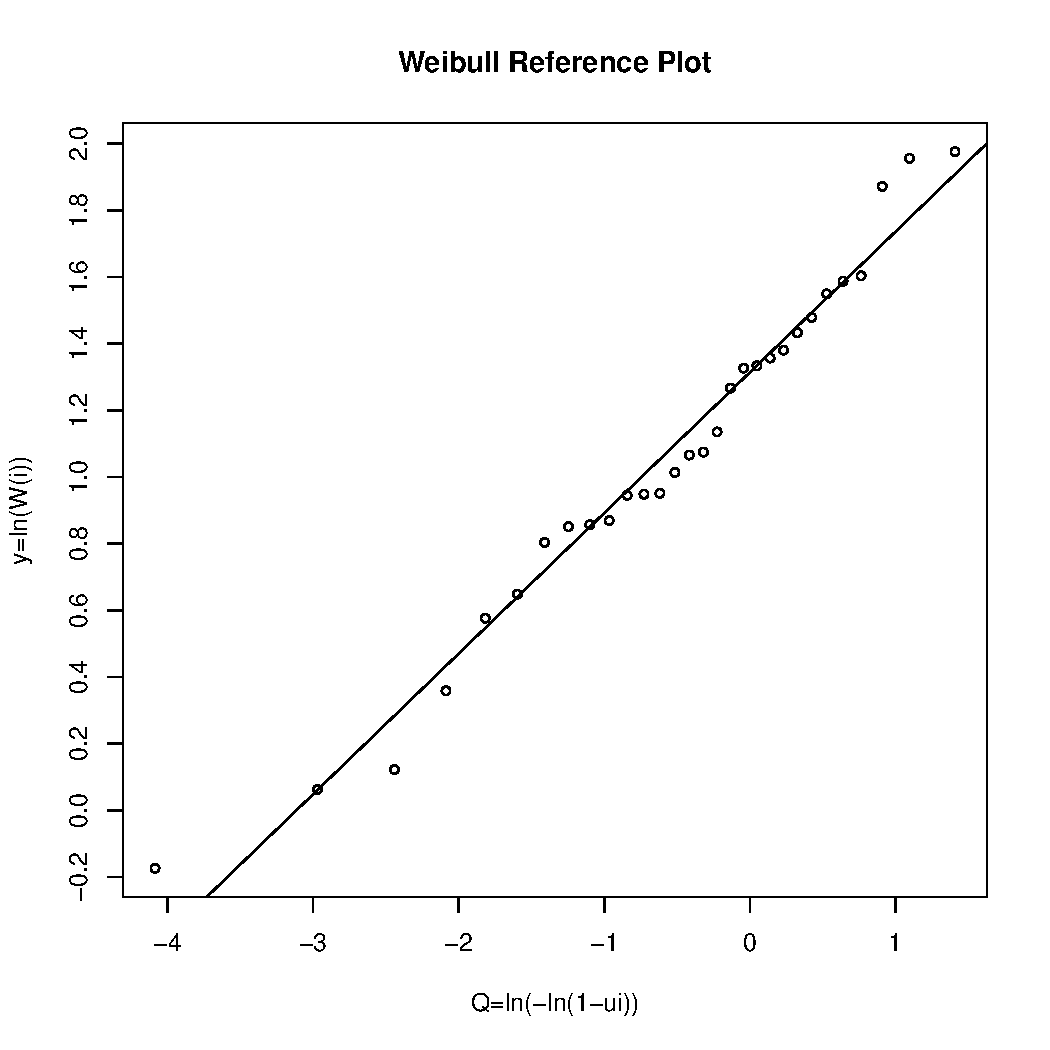
\includegraphics[width=0.8\textwidth]{Rplots.pdf}
\end{figure}
\newpage
We will also compute the Anderson-Darling GOF test in R: \\
\begin{verbatim}
library(MASS)
mle <- fitdistr(x,"weibull")
shape = mle$estimate[1]
scale = mle$estimate[2]
a = -log(scale)
b = 1/shape
z = exp(-exp(-(y-a)/b))
A1i = (2*i-1)*log(z)
A2i = (2*n+1-2*i)*log(1-z)
s1 = sum(A1i)
s2 = sum(A2i)
AD = -n-(1/n)*(s1+s2)
ADM = AD*(1+.2/sqrt(n))
AD
ADM
\end{verbatim}
This results in $A^2 = 0.3059062$. From the table in Handout 9, this corresponds with a p-value > .25. Combining this with the fact that the reference plot is fairly straight, I am inclined to say the Weibull distribution is a good fit for the data.
\end{enumerate}
\end{document}